% importa variabili globali
% definizione variabili globali
\def\GRUPPO {\textit{DazzleWorks}}

\def\PROGETTO {\textbf{Premi}}

\def\COMMITTENTE {Prof. Vardanega Tullio, \\ & Dr. Cardin Riccardo}

\def\EMAIL {dazzleworksgroup@gmail.com}

\def\LOGO {../../template/img/logo.png}

\def\INTESTAZIONE {../../template/img/intestazione.png}
\def\PIEDIPAGINA {../../template/img/piedipagina.png}

\def\G {{\small $_G$}}





% definizione variabili locali
\def\DOCUMENTO{Analisi dei Requisiti}
\def\VERSIONE{1.0.0}

\def\DESCRIZIONE{Documento che descrive l'analisi dei requisiti e dei casi d'uso del gruppo \GRUPPO per il progetto \PROGETTO}

\def\REDATTORE {Matteo Agostinetto \\ & Nicola Carraro}
\def\VERIFICATORE {<Verificatore>}
\def\RESPONSABILE {Valerio Burlin}

\def\USO {Esterno}

\def\DISTRIBUZIONE {\GRUPPO{}\\ & \COMMITTENTE{}\\}

\def\DESCRIZIONE {Documento che descrive l'analisi dei requisiti e dei casi d'uso del gruppo \GRUPPO per il progetto \PROGETTO}


% abilita (true) / disabilita (false) indice, lista tabelle, lista figure
\def\INDICE	{true}
\def\TABELLE {true}
\def\FIGURE {true}


% importa struttura
\documentclass[a4paper]{article}

% ----- definizioni -----
\def\TITLE		{\mbox{\GRUPPO}}
\def\SUBTITLE	{\SIGLA, \PROGETTO}


% ----- nuovi comandi -----
% fornisce il caption per riferirsi ad una particolare sezione
\newcommand{\numref}[1]{\textsf{\textsl{``\nameref{#1}'' (\ref{#1})}}}


% ----- package -----
\usepackage[T1]{fontenc}   % codifica dei font in uscita
\usepackage[utf8x]{inputenc}   % lettere accentate da tastiera
\usepackage[italian]{babel}   % lingua principale del documento
\usepackage[a4paper, top= 3cm, bottom= 3cm, left= 3cm, right= 3cm, bindingoffset= 5mm]{geometry} % impostazione margini

\usepackage{amssymb} %

\usepackage{booktabs} % comandi aggiuntivi per le tabelle

\usepackage{calc} % espressioni aritmetiche
\usepackage{caption} % descrizione figure, ecc
\usepackage{chapterbib} % inclusione delle bibliografie

\usepackage{datatool} % manipolazione dati
\usepackage{dcolumn} % array in tabular

\usepackage{epstopdf} % conversione eps--> pdf
\usepackage{enumitem} % personalizzazione liste
\usepackage{eurosym} % simbolo euro

\usepackage{fancyhdr}   %personalizzazione dello stile
\usepackage{float} % definizione di oggetti floating (es. figure, tabelle)
\usepackage[bottom]{footmisc} % personalizzazione note

\usepackage[toc]{glossaries}	% glossario
\usepackage{graphicx, subfigure} % pacchetto grafica testo
\usepackage{grffile} % estende gestione filename graphic

\usepackage[colorlinks=true, urlcolor=blue, citecolor=black, linkcolor=black, hyperindex, breaklinks]{hyperref} % gestione dei link

\usepackage{ifthen}	% costrutto ifthenelse

% \usepackage{listings} % inserimento pezzi di codice
\usepackage{longtable} % tabelle su più pagine

\usepackage{pgf} % grafica postscript e PDF
\usepackage{pgfplots}	% composizione di grafici
\pgfplotsset{/pgf/number format/use comma, compat=newest}	% opzioni per i grafici

\usepackage{multirow} % span multiriga

\usepackage{tabularx, array} % crea paragrafi a colonne
\usepackage{titlesec} % personalizzazione titoli
\usepackage{tikz} % gestione delle formule
\usepackage{totpages} % conta numero pagine

\usepackage{soul} % gestione letterspacing
\usepackage{subfigure} % gestione delle sottofigure

\usepackage{verbatim} % inserimento testo verbatim, non interpretato

\usepackage{wallpaper} % gestione background

\usepackage{xspace} % spazi automatici per le macro


% ----- posizione etichette -----
\captionsetup{tableposition=top, figureposition=bottom, font=small}


% ----- glossario -----
\loadglsentries{../../glossario/glossario.tex}
\renewcommand*{\glssymbolsgroupname}{Simboli}


% ----- stile pagina -----
\pagestyle{fancy}

	% header
	\fancypagestyle {firststyle} {	% definizione stile "firststyle"
		\fancyhf{}
	}

	% indentazione paragrafo
	%\setlength{\parindent} {0pt}
	\setlength{\headheight} {25pt}

	% intestazione
	\lhead{}
	\rhead{\nouppercase{\leftmark}}
	\renewcommand{\headrulewidth}{0pt}  % no linea sotto intestazione

	% piè di pagina
	\lfoot{\footnotesize{{\DOCUMENTO} \\ {\VERSIONE}}}
	\cfoot{}
	\rfoot{\thepage}
	\renewcommand{\footrulewidth}{0pt}   % no linea sopra piè di pagina


% ----- inizio documento -----
% ----- prima pagina -----
\begin{document}
\thispagestyle{firststyle}

\begin{center}

%   \vspace{7cm}
	\textbf{{\fontsize{40pt}{41pt}\selectfont \PROGETTO}} \\
	\rule{8cm}{3pt}
   
   \vspace{4cm}
   \includegraphics[height= 4cm] {\LOGO}
   
	\vspace{1cm}
   {\fontsize{30pt}{31pt}\selectfont \textbf{\GRUPPO}}
	
	\vspace{5cm}
	{\fontsize{18pt}{24pt}\selectfont \textbf{\DOCUMENTO}}
	
%	\vspace{1cm}
	\begin{center}
		\begin{tabular}{r|l}
				\textbf{Versione} & \VERSIONE \\
				\textbf{Redattori} & \REDATTORE \\
				\textbf{Verificatori} & \VERIFICATORE \\
				\textbf{Responsabili} & \RESPONSABILE \\
				\textbf{Uso} & \USO \\
				\textbf{Lista di distribuzione} & \DISTRIBUZIONE
		\end{tabular}
	\end{center}

	\vspace{1cm}
	\textbf{\DESCRIZIONE}

\end{center}


\newpage

% ----- pagine successive -----
\ULCornerWallPaper{1}{\INTESTAZIONE}
\LLCornerWallPaper{1}{\PIEDIPAGINA}

%\thispagestyle{empty}

\newpage

% diario delle modifiche


% numerazione pagine indici
\pagenumbering{Roman}



% importa indici
% definizione indice
\ifthenelse{\equal{\INDICE}{true}}
	{\tableofcontents \newpage}{}

% definizione lista tabelle
%\ifthenelse{\equal{\TABELLE}{true}} 
%	{\listoftables \newpage}{}

% definizione lista figure
\ifthenelse{\equal{\FIGURE}{true}}
	{\listoffigures \newpage}{}


% numerazione pagine
\pagenumbering{arabic}

	% formato visualizzazione
	\rfoot{\thepage ~di~\pageref{TotPages}}


% separatore
\iffalse
	AOjvdYTJD7mcIIYItfsNiYPbmTTogRSP9hrrb2XPE1laMyQ9NHrPgTCTxnW0eV1YcM3Wqh7t5qThjczeXWq3O5FJ7BBQjoWZovC5
\fi


% importa parti documento

%\section{<nomesezione>}
%\input{sections/<nomefile>.tex}

%\newpage

\section{Introduzione}
\subsection{Scopo del documento}
Il \textit{Piano di Qualifica} ha lo scopo di fissare le strategie che il gruppo intende adottare, al fine di perseguire gli obbiettivi di qualità, sia di processo che di prodotto. Per questo motivo è necessaria una costante verifica sulle attività svolte. Così facendo si permette di trovare possibili incongruenze e anomalie per poter intervenire in maniera tempestiva ed efficace.
\subsection{Scopo del prodotto}
Lo scopo del prodotto è la realizzazione di un software di presentazione di \textit{slide}, utilizzando il linguaggio HTML5, che funzioni sia su desktop che su dispositivi mobile. Si richiede di realizzare effetti grafici a supporto dello \textit{storytelling}\footnote{L'arte del raccontare storie impiegata come strategia di comunicazione.} e che sia di livello comparabile con Prezi\footnote{Software di presentazioni.}.
\subsection{Glossario}
Al fine di evitare ogni ambiguità e permettere al lettore una migliore comprensione i termini tecnici e gli acronimi sono riportati, con relativa descrizione, nel documento \textit{Glossario}. 
Ogni occorrenza di un termine appartenente al \textit{Glossario} è marcata da una \G in pedice.
\subsection{Riferimenti}
	\subsubsection{Normativi}
	\begin{itemize}
		\item \textbf{Norme di Progetto:} \textit{Norme di Progetto v1.0.0};
		\item \textbf{Capitolato d'appalto C4:} Premi: software di presentazione "better than Prezzi" \url{http://www.math.unipd.it/~tullio/IS-1/2014/Progetto/C4p.svg#1_0}.
	\end{itemize}
	\subsubsection{Informativi}
	\begin{itemize}
		\item \textbf{Piano di Progetto:} \textit{Piano di Progetto v1.0.0};
		\item \textbf{Slide Ingegneria del Software 2014/2015:} \url{http://www.math.unipd.it/~tullio/IS-1/2014/}
		\item \textbf{Indice Gulpease:} \url{http://it.wikipedia.org/wiki/Indice_Gulpease}
		\item \textbf{Standard ISO/IEC 9126:} \url{http://it.wikipedia.org/wiki/ISO/IEC_9126}
		\item \textbf{Standard ISO/IEC 15504:} \url{http://en.wikipedia.org/wiki/ISO/IEC_15504}
	\end{itemize}
\newpage

\section{Descrizione Generale}
\subsection{Prospettive d'uso del prodotto}
Il prodotto ha l'obbiettivo di fornire uno strumento in grado di creare una presentazione di slide, sviluppato in tecnologia HTML5 GLS??????, che risulti utilizzabile sia da piattaforme desktop che da mobile. Inoltre il prodotto garantirà l'inserimento di dati in \textit{real time}, ad esempio indici di borsa oppure link a immagini e video, rendendo le slide sempre aggiornate. Il software sarà disponibile per i maggiori sistemi operativi: Windows GLS????, Linux GLS????, MAC OS X GLS???.

\subsection{Funzioni del prodotto}
Il prodotto sfrutterà il browser GLS??? come GUI GLS???. Il programma in sè non andrà interpretato come una pagina web, ma come un software che per l'occasione utilizzi il linguaggio Javascript GLS???? e le librerie contenute nel browser GLS???.
Una volta avviato il programma sarà possibile:
\begin{itemize}
	\item Creare un nuovo progetto o caricare un progetto già esistente:
	\begin{itemize}
		\item Creare nuove slide;
		\item Modificare le slide precedentemente create;
		\item Cancellare slide;
		\item Scegliere effetti visivi di transizione;
		\item Inserire e posizionare del testo;
		\item Selezionare colore, font GLS???, e grandezza del testo;
		\item Inserire e posizionare una o più immagini;
		\item Inserire dati real time GLS????.
	\end{itemize}
	\item Salvare il progetto;
	\item Esportare il progetto;
	\item Stampare la presentazione creata:
	\begin{itemize}
		\item Stampare tutte le slide o solo alcune.
	\end{itemize}
	\item Creare un'infografica:
	\begin{itemize}
		\item Scegliere il layout GLS??? per l'infografica;
		\item Inserire il contenuto nell'infografica.
	\end{itemize}
	\item Stampare un'infografica.
\end{itemize}

\subsection{Caratteristiche dell'utente}
Non esiste una categoria di utenti definita ai quali sia rivolto il software, al giorno d'oggi infatti la presentazione tramite slide viene utilizzata da studenti, insegnanti, politici, rappresentanti, dottori e molti altri. Bisogna quindi essere in grado di fornire un prodotto di semplice utilizzo e intuitivo.

\subsection{Vincoli Generali}
Il software potrà essere eseguito su qualunque sistema operativo, ma avrà dei vincoli sul browser GLS??? da utilizzare, che sono i seguenti:
\begin{itemize}
	\item Google Chrome v??????
	\item Mozilla Firefox v?????????
	\item Internet Explorer v??????
	\item Opera v????????
	\item Safari v?????????
\end{itemize}
\newpage

\section{Casi d'uso}
Verrano descritti di seguito i casi d'uso individuati per il progetto \PROGETTO. Ogni caso d'uso ha un codice che lo indentifica nella forma:
\begin{center}
	UC[codice univoco del padre].[codice progressivo di livello]
\end{center}
Il codice progressivo di livello potrà contenere diversi altri livelli di gerarchia, essi saranno separati da un punto. Per comodità e chiarezza lo scenario principale verrà individuato attraverso il codice UCP. Successivamente verranno descritti i figli senza però riportare il codice del padre.

\subsection{Caso d'uso UCP: Scenario principale}
\begin{figure}[h] 
	\centering 
	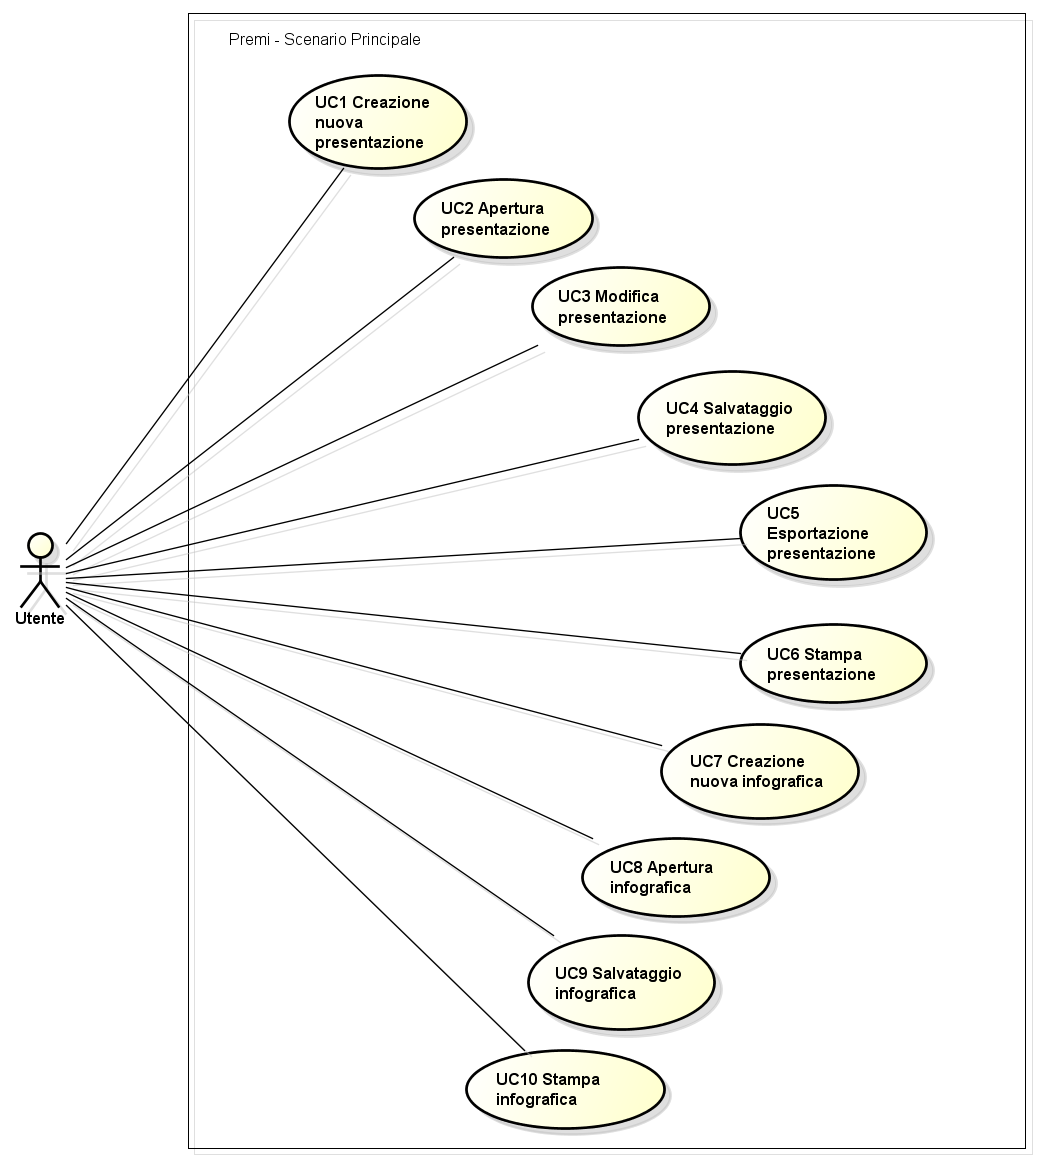
\includegraphics[scale=0.5] {img/UCP.png} 
	\caption{UCP - Scenario principale} 
\end{figure}

\newpage

\begin{itemize}
	\item \textbf{Attori:} Utente;
	\item \textbf{Scopo e descrizione:} Dopo aver avviato il programma, l'utente potrà effettuare diverse operazioni. Potrà creare una nuova presentazione o caricarne una precedentemente creata. Analogamente potrà creare una nuova infografica oppure caricarne una già creata. Se è aperta una presentazione o una infografica l'utente potrà modificare e salvare i nuovi cambiamenti o esportare l'intera presentazione (o infografica). Inoltre l'utente avrà a disposizione una funzione di stampa per stampare le slide della presentazione oppure l'infografica;
	\item \textbf{Precondizione:} Il programma è stato correttamente avviato ed è pronto all'uso;
	\item \textbf{Flusso degli eventi:}
	\begin{enumerate}
		\item L'utente può creare una nuova presentazione [UC1];
		\item L'utente può aprire una presentazione [UC2];
		\item L'utente può modificare una presentazione [UC3];
		\item L'utente può salvare una presentazione [UC4];
		\item L'utente può esportare una presentazione [UC5];
		\item L'utente può stampare una presentazione [UC6];
		\item L'utente può creare una nuova infografica [UC7];
		\item L'utente può aprire una infografica [UC8];
		\item L'utente può salvare una infografica [UC9];
		\item L'utente può stampare una infografica [UC10].
	\end{enumerate}
	\item \textbf{Postcondizione:} Il sistema ha ottenuto le informazioni sulle operazioni che l’utente desidera eseguire.
\end{itemize}

\subsection{Caso d'uso UC1: Creazione nuova presentazione}
\begin{figure}[h] 
	\centering 
	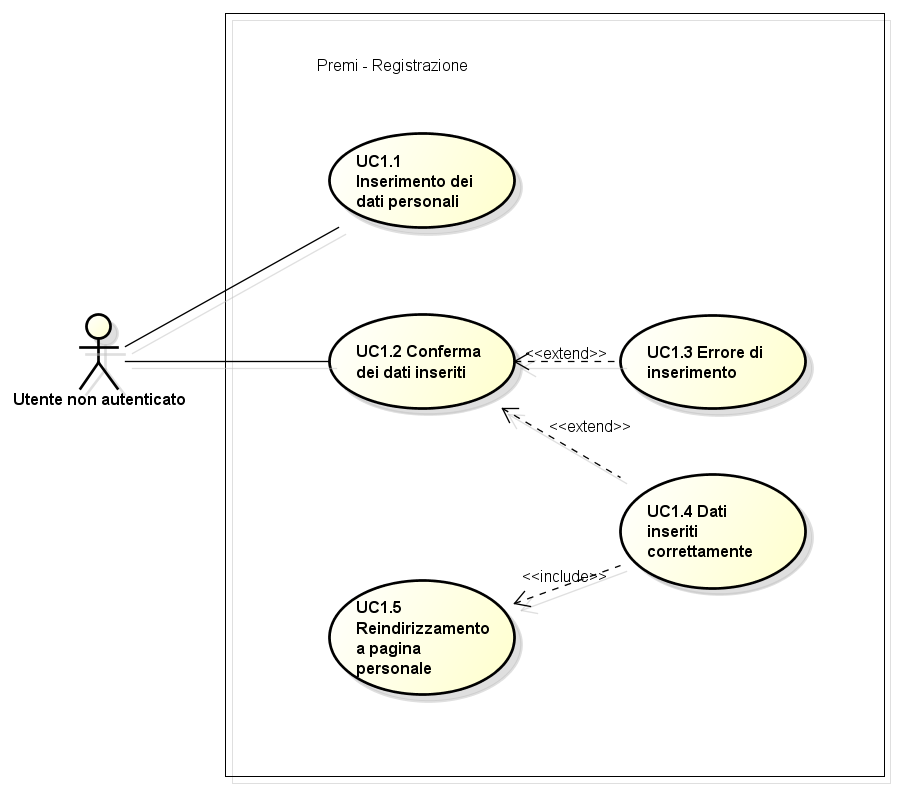
\includegraphics[scale=0.45] {img/UC1.png} 
	\caption{UC1 - Creazione nuova presentazione} 
\end{figure}

\begin{itemize}
	\item \textbf{Attori:} Utente;
	\item \textbf{Scopo e descrizione:} L'utente sta creando una nuova presentazione di slide. Per completare l'operazione deve inserire almeno una slide vuota. Potrà anche inserire una o più: immagine, casella di testo, dato real time. Potrà essere scelto anche l'effetto di transizione da una slide ad un'altra;
	\item \textbf{Precondizione:} Il sistema mostra la schermata di creazione di una presentazione e l'utente vuole creare una nuova slide;
	\item \textbf{Flusso degli eventi:}
	\begin{enumerate}
		\item L'utente crea una nuova slide [UC1.1];
		\item L'utente può inserire un'immagine o più [UC1.2];
		\item L'utente carica un file per inserire l'immagine [UC1.6];
		\item L'utente può inserire una casella di testo o più [UC1.3];
		\item L'utente sceglie la formattazione del testo [UC1.7];
		\item L'utente può inserire dei dati real time [UC1.4];
		\item L'utente può scegliere un effetto di transizione [UC1.5];
	\end{enumerate}
	\item \textbf{Postcondizione:} Il sistema mostra le operazioni effettuate dall'utente.
\end{itemize}

\subsection{Caso d'uso UC1.1: Inserire nuova slide}
\begin{itemize}
	\item \textbf{Attori:} Utente;
	\item \textbf{Scopo e descrizione:} L'utente crea una nuova slide nella presentazione per poter inserire del contenuto;
	\item \textbf{Precondizione:} Il sistema è in attesa che l'utente crei una nuova slide;
	\item \textbf{Postcondizione:} Il sistema ha creato la nuova slide.
\end{itemize}

\subsection{Caso d'uso UC1.2: Inserire un'immagine}
\begin{itemize}
\item \textbf{Attori:} Utente;
\item \textbf{Scopo e descrizione:} L'utente deve inserire l'immagine da mettere nella slide;
\item \textbf{Precondizione:} Il sistema è in attesa che l'utente selezioni l'immagine;
\item \textbf{Postcondizione:} Il sistema ha caricato l'immagine selezionata dall'utente.
\end{itemize}

\subsection{Caso d'uso UC1.3: Inserire casella di testo}
\begin{itemize}
\item \textbf{Attori:} Utente;
\item \textbf{Scopo e descrizione:} L'utente deve inserire una casella di testo nella slide;
\item \textbf{Precondizione:} Il sistema è in attesa che l'utente crei una casella di testo;
\item \textbf{Postcondizione:} Il sistema ha creato la casella di testo.
\end{itemize}

\subsection{Caso d'uso UC1.4: Inserire dati real time}
\begin{itemize}
	\item \textbf{Attori:} Utente;
	\item \textbf{Scopo e descrizione:} L'utente deve inserire dei dati real time;
	\item \textbf{Precondizione:} Il sistema è in attesa che l'utente inserisca i dati real time;
	\item \textbf{Postcondizione:} Il sistema ha inserito i dati real time.
\end{itemize}

\subsection{Caso d'uso UC1.5: Scegliere effetto di transizione}
\begin{itemize}
	\item \textbf{Attori:} Utente;
	\item \textbf{Scopo e descrizione:} L'utente deve scegliere l'effetto di transizione da dare alla slide;
	\item \textbf{Precondizione:} Il sistema è in attesa che l'utente selezioni l'effetto desiderato;
	\item \textbf{Postcondizione:} Il sistema ha inserito l'effetto di transizione.
\end{itemize}

\subsection{Caso d'uso UC1.6: Caricare file}
\begin{figure}[h] 
	\centering 
	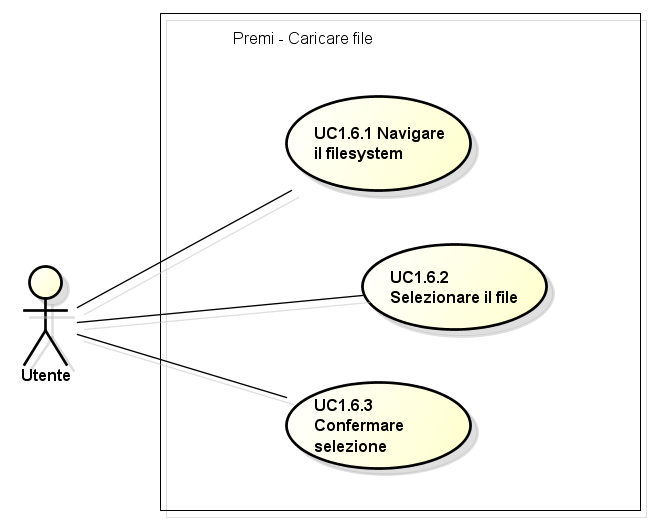
\includegraphics[scale=0.45] {img/UC1.6.png} 
	\caption{UC1.6 - Caricare file} 
\end{figure}

\begin{itemize}
	\item \textbf{Attori:} Utente;
	\item \textbf{Scopo e descrizione:} L'utente deve caricare un file. Naviga il filesystem cercando il file desiderato, lo seleziona e conferma la selezione caricando il file;
	\item \textbf{Precondizione:} Il sistema è in attesa che l'utente selezioni il file;
	\item \textbf{Flusso degli eventi:}
	\begin{enumerate}
		\item L'utente naviga il filesystem alla ricerca del file desiderato [UC1.6.1];
		\item L'utente seleziona il file [UC1.6.2];
		\item L'utente conferma il file selezionato [UC1.6.3].
	\end{enumerate}
	\item \textbf{Postcondizione:} Il sistema ha caricato il file selezionato dall'utente e lo ha inserito nella slide.
\end{itemize}

\subsection{Caso d'uso UC1.6.1: Navigare il filesystem}
\begin{itemize}
	\item \textbf{Attori:} Utente;
	\item \textbf{Scopo e descrizione:} L'utente può navigare il filesystem per selezionare la cartella dentro la quale è contenuto il file desiderato;
	\item \textbf{Precondizione:} Il sistema è in attesa che l'utente selezioni una cartella;
	\item \textbf{Postcondizione:} Il sistema ha aggiornato la cartella corrente con quella scelta dall'utente.
\end{itemize}

\subsection{Caso d'uso UC1.6.2: Selezionare il file}
\begin{itemize}
	\item \textbf{Attori:} Utente;
	\item \textbf{Scopo e descrizione:} L'utente deve selezionare il file che intende caricare;
	\item \textbf{Precondizione:} Il sistema mostra i file contenuti nella cartella precedentemente selezionata;
	\item \textbf{Postcondizione:} Il sistema evidenzia il file scelto dall'utente.
\end{itemize}

\subsection{Caso d'uso UC1.6.3: Confermare selezione}
\begin{itemize}
	\item \textbf{Attori:} Utente;
	\item \textbf{Scopo e descrizione:} L'utente conferma che il file selezionato in precedenza è quello corretto;
	\item \textbf{Precondizione:} Il sistema ha selezionato il file indicato dall'utente;
	\item \textbf{Postcondizione:} Il sistema ha caricato il file scelto precedentemente dall'utente.
\end{itemize}

\subsection{Caso d'uso UC1.7: Scegliere formattazione del testo}
\begin{figure}[h] 
	\centering 
	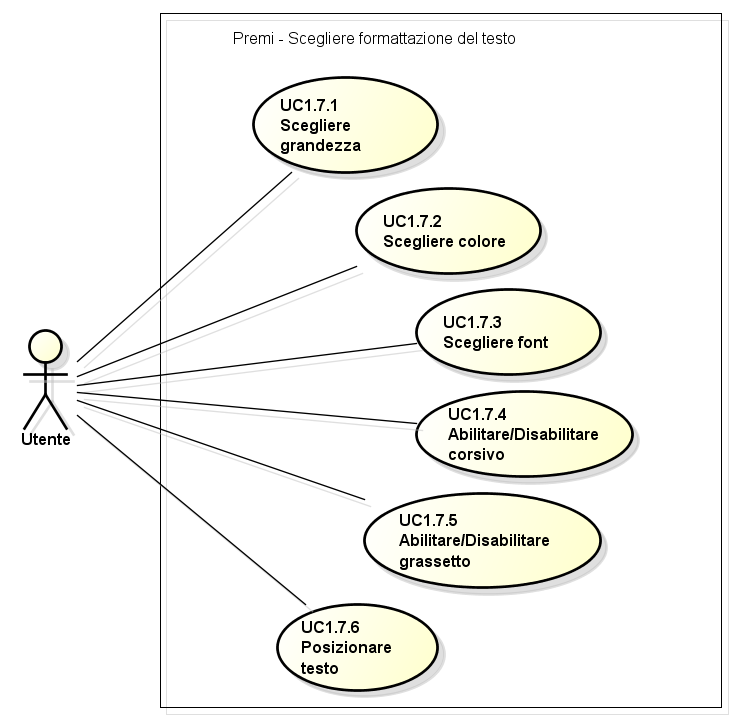
\includegraphics[scale=0.45] {img/UC1.7.png} 
	\caption{UC1.7 - Scegliere formattazione del testo} 
\end{figure}

\begin{itemize}
	\item \textbf{Attori:} Utente;
	\item \textbf{Scopo e descrizione:} L'utente può modificare l'aspetto del testo contenuto in una casella di testo. L'utente seleziona il testo e poi sceglie che modifiche effettuare;
	\item \textbf{Precondizione:} Il sistema è in attesa che l'utente selezioni la modifica da apportare al testo e il testo da modificare è selezionato;
	\item \textbf{Flusso degli eventi:}
	\begin{enumerate}
		\item L'utente può cambiare la grandezza del testo [UC1.7.1];
		\item L'utente può cambiare il colore del testo [UC1.7.2];
		\item L'utente può cambiare il font del testo [UC1.7.3];
		\item L'utente può abilitare o disabilitare il testo in corsivo [UC1.7.4];
		\item L'utente può abilitare o disabilitare il testo in grassetto [UC1.7.5];
		\item L'utente può spostare il testo in una nuova posizione [UC1.7.6].
	\end{enumerate}
	\item \textbf{Postcondizione:} Il sistema ha apportato le modifiche scelte al testo.
\end{itemize}

\subsection{Caso d'uso UC1.7.1: Scegliere grandezza}
\begin{itemize}
	\item \textbf{Attori:} Utente;
	\item \textbf{Scopo e descrizione:} L'utente può cambiare la grandezza del testo;
	\item \textbf{Precondizione:} Il testo da modificare è selezionato;
	\item \textbf{Postcondizione:} Il testo è stato ingrandito o rimpicciolito secondo la scelta dell'utente.
\end{itemize}

\subsection{Caso d'uso UC1.7.2: Scegliere colore}
\begin{itemize}
	\item \textbf{Attori:} Utente;
	\item \textbf{Scopo e descrizione:} L'utente può cambiare il colore del testo;
	\item \textbf{Precondizione:} Il testo da modificare è selezionato;
	\item \textbf{Postcondizione:} Il testo è stato colorato secondo la scelta dell'utente.
\end{itemize}

\subsection{Caso d'uso UC1.7.3: Scegliere font}
\begin{itemize}
	\item \textbf{Attori:} Utente;
	\item \textbf{Scopo e descrizione:} L'utente può cambiare il font del testo;
	\item \textbf{Precondizione:} Il testo da modificare è selezionato;
	\item \textbf{Postcondizione:} Il testo ha cambiato font secondo la scelta dell'utente.
\end{itemize}

\subsection{Caso d'uso UC1.7.4: Abilitare/Disabilitare corsivo}
\begin{itemize}
	\item \textbf{Attori:} Utente;
	\item \textbf{Scopo e descrizione:} L'utente può abilitare o disabilitare la scrittura in corsivo;
	\item \textbf{Precondizione:} Il testo da modificare è selezionato oppure è stata selezionata la casella di testo nella quale poter scrivere;
	\item \textbf{Postcondizione:} Il testo è stato modificato secondo la scelta dell'utente.
\end{itemize}

\subsection{Caso d'uso UC1.7.5: Abilitare/Disabilitare grassetto}
\begin{itemize}
	\item \textbf{Attori:} Utente;
	\item \textbf{Scopo e descrizione:} L'utente può abilitare o disabilitare la scrittura in grassetto;
	\item \textbf{Precondizione:} Il testo da modificare è selezionato oppure è stata selezionata la casella di testo nella quale poter scrivere;
	\item \textbf{Postcondizione:} Il testo è stato modificato secondo la scelta dell'utente.
\end{itemize}

\subsection{Caso d'uso UC1.7.6: Posizionare testo}
\begin{itemize}
	\item \textbf{Attori:} Utente;
	\item \textbf{Scopo e descrizione:} L'utente può spostare una casella di testo in una nuova posizione;
	\item \textbf{Precondizione:} La casella di testo da spostare è stata selezionata;
	\item \textbf{Postcondizione:} La casella di testo è stata spostata secondo la scelta dell'utente.
\end{itemize}


\newpage
% ...

%\printglossaries

\end{document}
